\textbf{See the instruction for questions \inteval{\value{question}+1} to \inteval{\value{question}+2}.}

\begin{figure}[H]
    \centering
    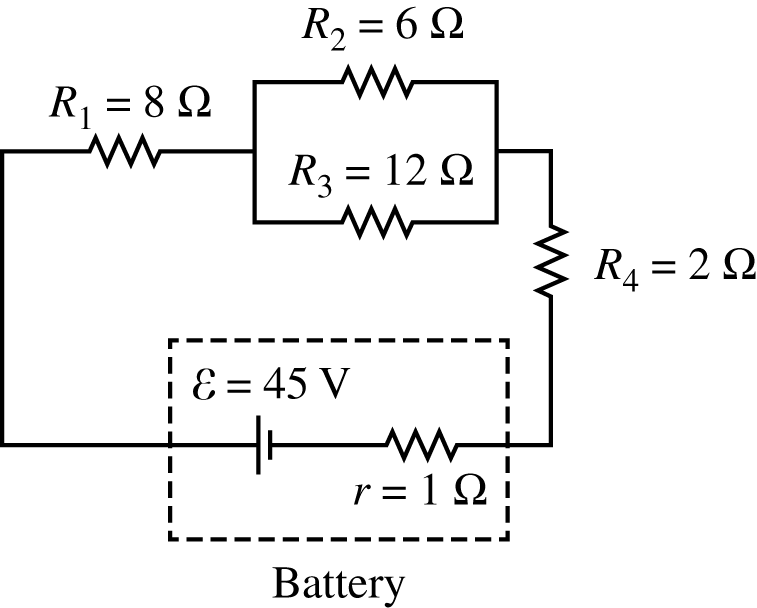
\includegraphics[scale=0.3]{images/img-011-026.png}
\end{figure}

The circuit represented in the figure above contains four resistors and a battery. The $45 \unit{V}$ battery has a $1 \latinunit\Omega$ internal resistance.

% Multiple Choice Question 24
\begin{questions}\setcounter{question}{23}\question
Which of the following ranks the absolute values of the potential differences $\Delta V$ across the resistors from highest to lowest?

\begin{choices}
\choice $\Delta V_{3}>\Delta V_{1}>\Delta V_{2}>\Delta V_{4}$
\choice $\Delta V_{4}>\Delta V_{2}>\Delta V_{1}>\Delta V_{3}$
\choice $\Delta V_{1}>\Delta V_{4}>\Delta V_{2}>\Delta V_{3}$
\choice $\Delta V_{1}>\left(\Delta V_{2}=\Delta V_{3}\right)>\Delta V_{4}$
\choice $\Delta V_{4}>\left(\Delta V_{2}=\Delta V_{3}\right)>\Delta V_{1}$
\end{choices}\end{questions}

% Multiple Choice Question 25
\begin{questions}\setcounter{question}{24}\question
How much energy is dissipated by the battery's internal resistance in $60 \unit{s}$ ?

\begin{oneparchoices}
\choice $9 \unit{J}$
\choice $180 \unit{J}$
\choice $540 \unit{J}$
\choice $900 \unit{J}$
\choice $8100 \unit{J}$
\end{oneparchoices}\end{questions}
